
\chapter{Pendolo su carrello}
\section{Equazioni e linearizzazione del modello}

\begin{center}
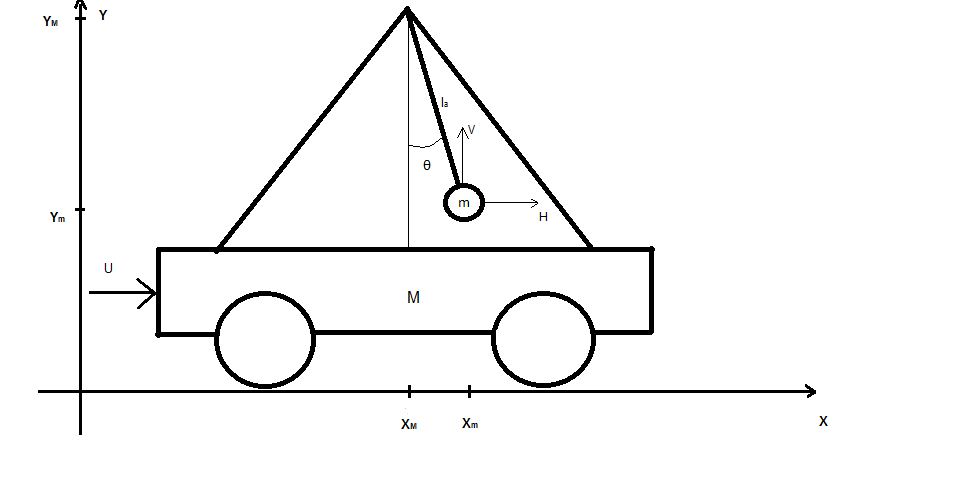
\includegraphics[scale=0.6]{pendolo.png}
\end{center}
Modello del pendolo su carrello realizzato con LEGO MINDSTORM EV3\\\\
\textbf{Bilanciamento forse sull'asta}\\
Asse x:
\begin{equation}
m\ddot{x}_m=H
\end{equation}
Asse y:
\begin{equation}
m\ddot{y}_m=V-mg
\end{equation}
Avendo:\\
\begin{equation}
x_m = x_M+l_a\sin(\theta) \quad \Rightarrow \quad \ddot{x}_m=\ddot{x}_M-l_a\sin(\theta)\dot{\theta}^2+l_a\cos(\theta)\ddot{\theta}
\end{equation}
\begin{equation}
y_m=y_F-l_a\cos(\theta) \quad \Rightarrow \quad \ddot{y}_m=l_a(\ddot{\theta}\sin(\theta)+\dot{\theta}^2\cos(\theta))
\end{equation}
Si ottiene:
\begin{equation}\label{H}
H=m\ddot{x}_M-ml_a\sin(\theta)\dot{\theta}^2+ml_a\cos(\theta)\ddot{\theta}
\end{equation}
\begin{equation}\label{V}
V=mg+ml_a\cos(\theta)\dot{\theta}^2+ml_a\sin(\theta)\ddot{\theta}
\end{equation}
\textbf{Bilanciamento forze sul carrello}
\begin{equation}
M\ddot{x}_M=u-H
\end{equation}
sostituendo la \ref{H} si ha:
$$
M\ddot{x}_M=u-m\ddot{x}_M+ml_a\sin(\theta)\dot{\theta}^2-ml_a\cos(\theta)\ddot{\theta}
$$
\begin{equation}\label{FCarr}
	(M+m)\ddot{x}_M+ml_a\cos(\theta)\ddot{\theta}=u+ml_a\dot{\theta}^2\sin(\theta)
\end{equation} 
\textbf{Bilanciamento momenti del sistema asta-massa}
\begin{equation}
I_m\ddot{\theta}=l_aV\sin(\theta)+l_aH\cos(\theta)
\end{equation}
sostituendo la \ref{H} e la \ref{V}:
$$
I_m\dot{\theta}=l_a\sin(\theta)[mg+ml_a\cos(\theta)\dot{\theta}^2+ml_a\sin(\theta)\ddot{\theta}]+l_a\cos(\theta)[m\ddot{x}_M-ml_a\sin(\theta)\dot{\theta}^2+ml_a\cos(\theta)\ddot{\theta}]=
$$
$$
=mgl_a\sin(\theta)+ml_a^2\sin(\theta)\cos(\theta)\dot{\theta}^2+ml_a^2\sin^2(\theta)\ddot{\theta}+ml_a\ddot{x}_M\cos(\theta)-ml_a^2\cos(\theta)\sin(\theta)\dot{\theta}^2$$
$$+ml_a^2\cos^2(\theta)\ddot{\theta}=$$
$$=mgl_a\sin(\theta)+ml_a^2\ddot{\theta}+ml_a\ddot{x}_M\cos(\theta) =
$$
\begin{equation} \label{momInThetaP}
=ml_a(g\sin(\theta)+l_a\ddot{\theta}+\ddot{x}_M\cos(\theta))
\end{equation}
Il sistema che deriva dalla \ref{FCarr} e dalla \ref{momInThetaP} è dunque il seguente:
\\\\
$\begin{cases}
$$(M+m)\ddot{x}_M+ml_a\cos(\theta)\ddot{\theta}=u+ml_a\dot{\theta}^2\sin(\theta)$$ \\
$$ml_a(g\sin(\theta)+l_a\ddot{\theta}+\ddot{x}_M\cos(\theta))$$\\
\end{cases}
$
\\\\\\
Assegno le variabili di stato:\\\\
$\begin{cases}
$$x_1 = x_M$$ \\
$$x_2=\dot{x}_M$$\\
$$x_3=\theta$$\\
$$x_4=\dot{\theta}$$\\
\end{cases}
$\\\\\\\
Dalla \ref{FCarr} si ottiene:
$$
\ddot{x}_M=\displaystyle\frac{u+ml_a\dot{\theta}^2\sin(\theta)-ml_a\cos(\theta)\ddot{\theta}}{M+m}
$$
$$
\ddot{\theta}=\displaystyle\frac{(M+m)I_m\dot{\theta}-g\sin(\theta)ml_a(M+m)-\cos(\theta)ml_au-\cos(\theta)\sin(\theta)\dot{\theta}^2m^2l_a^2+m^2l_a^2\cos^2(\theta)\ddot{\theta}}{ml_a^2(m+M)}
$$
\\
Le derivate prime delle variabili di stato del sistema sono dunque:
\\\\\\
$\begin{cases}
$$\dot{x}_1=\displaystyle\frac{u+ml_a\dot{\theta}^2\sin(\theta)-ml_a\cos(\theta)\ddot{\theta}}{M+m}$$ \\
$$\dot{x}_2=\dot{x}_M$$\\
$$\dot{x}_3=x_4$$\\
$$\dot{x}_4=\displaystyle\frac{(M+m)I_m\dot{\theta}-g\sin(\theta)ml_a(M+m)-\cos(\theta)ml_au-\cos(\theta)\sin(\theta)\dot{\theta}^2m^2l_a^2+m^2l_a^2\cos^2(\theta)\ddot{\theta}}{ml_a^2(m+M)}$$\\
\end{cases}
$
\\\\\\
\textbf{Punti di equilibrio del sistema} \\
Vogliamo ora linearizzare le precedenti equazioni di stato attorno al punto di equilibrio $\underline{x}=\underline{0}$, $u=0$ trovato: \\\\
$\displaystyle\frac{\partial{f_1}}{\partial{\underline{x}}}(\underline x)=
\begin{bmatrix}
0&1&0&0
\end{bmatrix}$\\\\\\
$\displaystyle\frac{\partial{f_2}}{\partial{x_1}}(\underline{x})=0$\quad
$\displaystyle\frac{\partial{f_2}}{\partial{x_2}}(\underline{x})=0$\quad
$\displaystyle\frac{\partial{f_2}}{\partial{x_3}}(\underline{x})=\displaystyle\frac{ml_ax_4^2\cos(x_3)+ml_a\sin(x_3)\dot{x_4}}{M+m}$\\
$\displaystyle\frac{\partial{f_2}}{\partial{x_4}}(\underline{x})=\displaystyle\frac{2ml_ax_4\sin(x_3)-ml_a\cos(x_3)\ddot{x_4}}{M+m}$\\\\\\
$\displaystyle\frac{\partial{f_3}}{\partial{\underline{x}}}(\underline x)=
\begin{bmatrix}
0&0&0&1
\end{bmatrix}$\\\\\\
$\displaystyle\frac{\partial{f_4}}{\partial{x_1}}(\underline{x})=0$\quad
$\displaystyle\frac{\partial{f_4}}{\partial{x_2}}(\underline{x})=0$\\
$\displaystyle\frac{\partial{f_4}}{\partial{x_3}}(\underline{x})=\displaystyle\frac{(ml_a)[-g\cos(x_3)(M+m)+\sin(x_3)u-2\cos(x_3)\sin(x_3)\dot{x_4}ml_a+(\sin^2(x_3)-cos^2(x_3))x^2_4ml_a]}{ml_a^2(M+m)}$\quad
$\displaystyle\frac{\partial{f_4}}{\partial{x_4}}(\underline{x})=\displaystyle\frac{(M+m)I_m-2\cos(x_3)\sin(x_3)x_4m^2l_a^2+m^2l_a^2\cos^2(x_3)\ddot{x_4}}{ml_a(M+m)}$\\\\
$\displaystyle\frac{\partial{f_1}}{\partial{u}}(\underline{x})=0$\quad
$\displaystyle\frac{\partial{f_2}}{\partial{u}}(\underline{x})=\displaystyle\frac{1}{M+m}$\quad
$\displaystyle\frac{\partial{f_3}}{\partial{u}}(\underline{x})=0$\quad
$\displaystyle\frac{\partial{f_4}}{\partial{u}}(\underline{x})=\displaystyle\frac{-\cos(x_3)}{l_a(M+m)}$\\\\
Sostituendo quindi nelle precedenti equazioni il punto di equilibrio si ottiene:\\\\
$\underline{\delta\dot{x}}=
\begin{bmatrix}
0&1&0&0\\
0&0&0&0\\
0&0&0&1\\
0&0&\displaystyle\frac{-g}{l_a}&\displaystyle\frac{I_m}{ml_a^2}
\end{bmatrix}
\underline{\delta x}+
\begin{bmatrix}
0\\
\displaystyle\frac{1}{M+m}\\
0\\
\displaystyle\frac{-1}{l_a(M+m)}\\
\end{bmatrix}
\underline{\delta u}
$\\\\
$\underline{\delta y}=
\begin{bmatrix}
1&0&0&0\\
0&0&1&0
\end{bmatrix}
\underline{\delta x}
$\\\\\\
Calcolando ora la funzione di Trasferimento $T(s)$ tra l'ingresso $u$(Forza esercitata sul carrello,
avanti/indietro) e l'uscita $y_2$(angolo $\theta$ del pendolo rispetto alla verticale) si ottiene:\\\\
$T_{u,y_2}(s)=C(sI-A)^{-1}B=
\begin{bmatrix}
0&0&1&0
\end{bmatrix}
\begin{bmatrix}
*&*&*&*\\
*&*&*&*\\
*&0&*&\displaystyle\frac{1}{s^2-\frac{I_m}{ml_a^2}s+\frac{g}{l_a}}\\
*&*&*&*
\end{bmatrix}
\begin{bmatrix}
0\\
\displaystyle\frac{1}{M+m}\\
0\\
\displaystyle\frac{-1}{l_a(M+m)}\\
\end{bmatrix} = \\
=\displaystyle\frac{-1}{l_a(M+m)(s^2-\frac{I_m}{ml_a^2}s+\frac{g}{l_a})}
$



